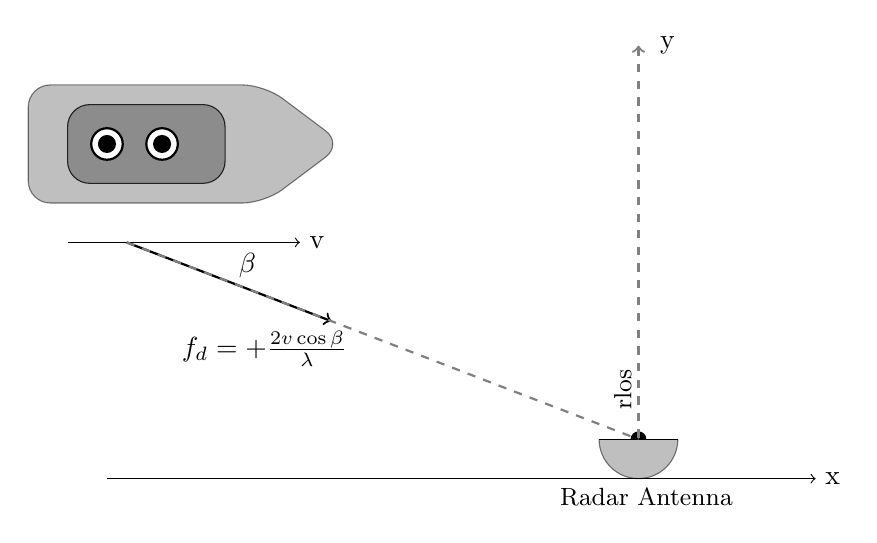
\begin{tikzpicture}
    % Boat 1
    \fill[gray, opacity=0.5, rounded corners=8pt, draw=black] (0,0) -- (3,0) -- (4,0.75) -- (3,1.5) -- (0,1.5) -- cycle;
    \fill[gray, opacity=0.8, rounded corners=8pt, draw=black] (0.5,0.25) rectangle (2.5,1.25);
    \fill[white, thick, draw=black] (1,0.75) ellipse (0.2 and 0.2);
    \fill[black, thick, draw=black] (1,0.75) ellipse (0.1 and 0.1);
    \fill[white, thick, draw=black] (1.7,0.75) ellipse (0.2 and 0.2);
    \fill[black, thick, draw=black] (1.7,0.75) ellipse (0.1 and 0.1);
    
    % Add velocity arrow for Boat 1
    \draw[->] (0.5,-0.5) -- (3.45,-0.5) node[right] {v};
    \draw[->, thick] (1.25,-0.5) -- (3.85,-1.5); \node[below] at (3,-1.5) {$f_d = +\frac{2v\cos\beta}{\lambda}$};
    \node[right] at (2.55,-0.8) {$\beta$};
    
    % Antenna
    \fill[gray, opacity = 0.5, -, draw = black] (7.25,-3) arc (180:360:0.5cm);
    \draw[-] (7.25,-3) -- (8.25,-3); % Optional: Draw a diameter (dashed line)
    \fill[-] (7.85,-3) arc (0:180:0.1cm);
    \node[below, font=\small] at (7.85,-3.5) {Radar Antenna};
    % Axis line
    \draw[->] (1,-3.5) -- (10,-3.5); \node[right] at (10,-3.5) {x};
    % RLOS lines
    %\draw[<-, dashed, thick, gray] (7.75,2) -- (7.75,-3); \node[right] at (7.9,2) {y};
    \draw[<-, thick, dashed, gray] (7.75,2) -- (7.75,-3); \node[right] at (7.9,2) {y};
    \draw[-, thick, dashed, gray] (1.25,-0.5) -- (7.75,-3);
    \node[right, rotate=90, font=\small] at (7.55,-2.75) {\gls{rlos}};
    
\end{tikzpicture}